\chapter{Sprint 3 : Communication, Administration et IA} 
\minitoc
\newpage

\section{Introduction}
Après avoir livré les fondations techniques (Sprint 1) et le cœur métier fonctionnel (Sprint 2), ce troisième et dernier sprint vient parachever la plateforme "CoachingApp". L'objectif est de transformer un simple outil de suivi en une véritable plateforme interactive et intelligente. Ce chapitre détaille l'implémentation de trois composants majeurs : la messagerie instantanée en temps réel pour renforcer le lien social entre coachs et athlètes, le développement du tableau de bord d'administration web en Angular, et enfin, l'intégration innovante de l'Intelligence Artificielle (via l'API Gemini) pour assister les utilisateurs au quotidien.

\section{Objectifs et Planification du Sprint}
\subsection{Backlog du Sprint 3}
Les tâches clôturant le cycle de développement sont :
\begin{itemize}
    \item \textbf{Tâche Backend 3.1 :} Implémenter le serveur WebSockets avec \texttt{Socket.io} pour gérer la messagerie bidirectionnelle en temps réel.
    \item \textbf{Tâche Backend 3.2 :} Configurer l'intégration avec Firebase Cloud Messaging (FCM) pour l'envoi de notifications push asynchrones.
    \item \textbf{Tâche Backend 3.3 :} Développer un wrapper pour l'API Google Gemini afin de générer des conseils d'entraînement via des requêtes de \textit{Prompt Engineering}.
    \item \textbf{Tâche Frontend (Flutter) 3.1 :} Créer l'interface de messagerie avec un design de type "Chat Bubbles" et gérer les événements de socket.
    \item \textbf{Tâche Web (Angular) 3.1 :} Développer le tableau de bord administrateur (Sidebar, KPI Cards, DataTable des utilisateurs).
\end{itemize}

\section{Conception détaillée du Sprint 3}

\subsection{Diagramme de cas d'utilisation (Sprint 3)}
Ce diagramme détaille les fonctionnalités avancées de la plateforme : la communication instantanée, l'administration globale par l'Admin, et la génération de recommandations par l'Intelligence Artificielle.

%[Note : Ajoutez l'image exportée depuis Draw.io dans le dossier diagrams/ avec ce nom]
\begin{figure}[H]
\centering
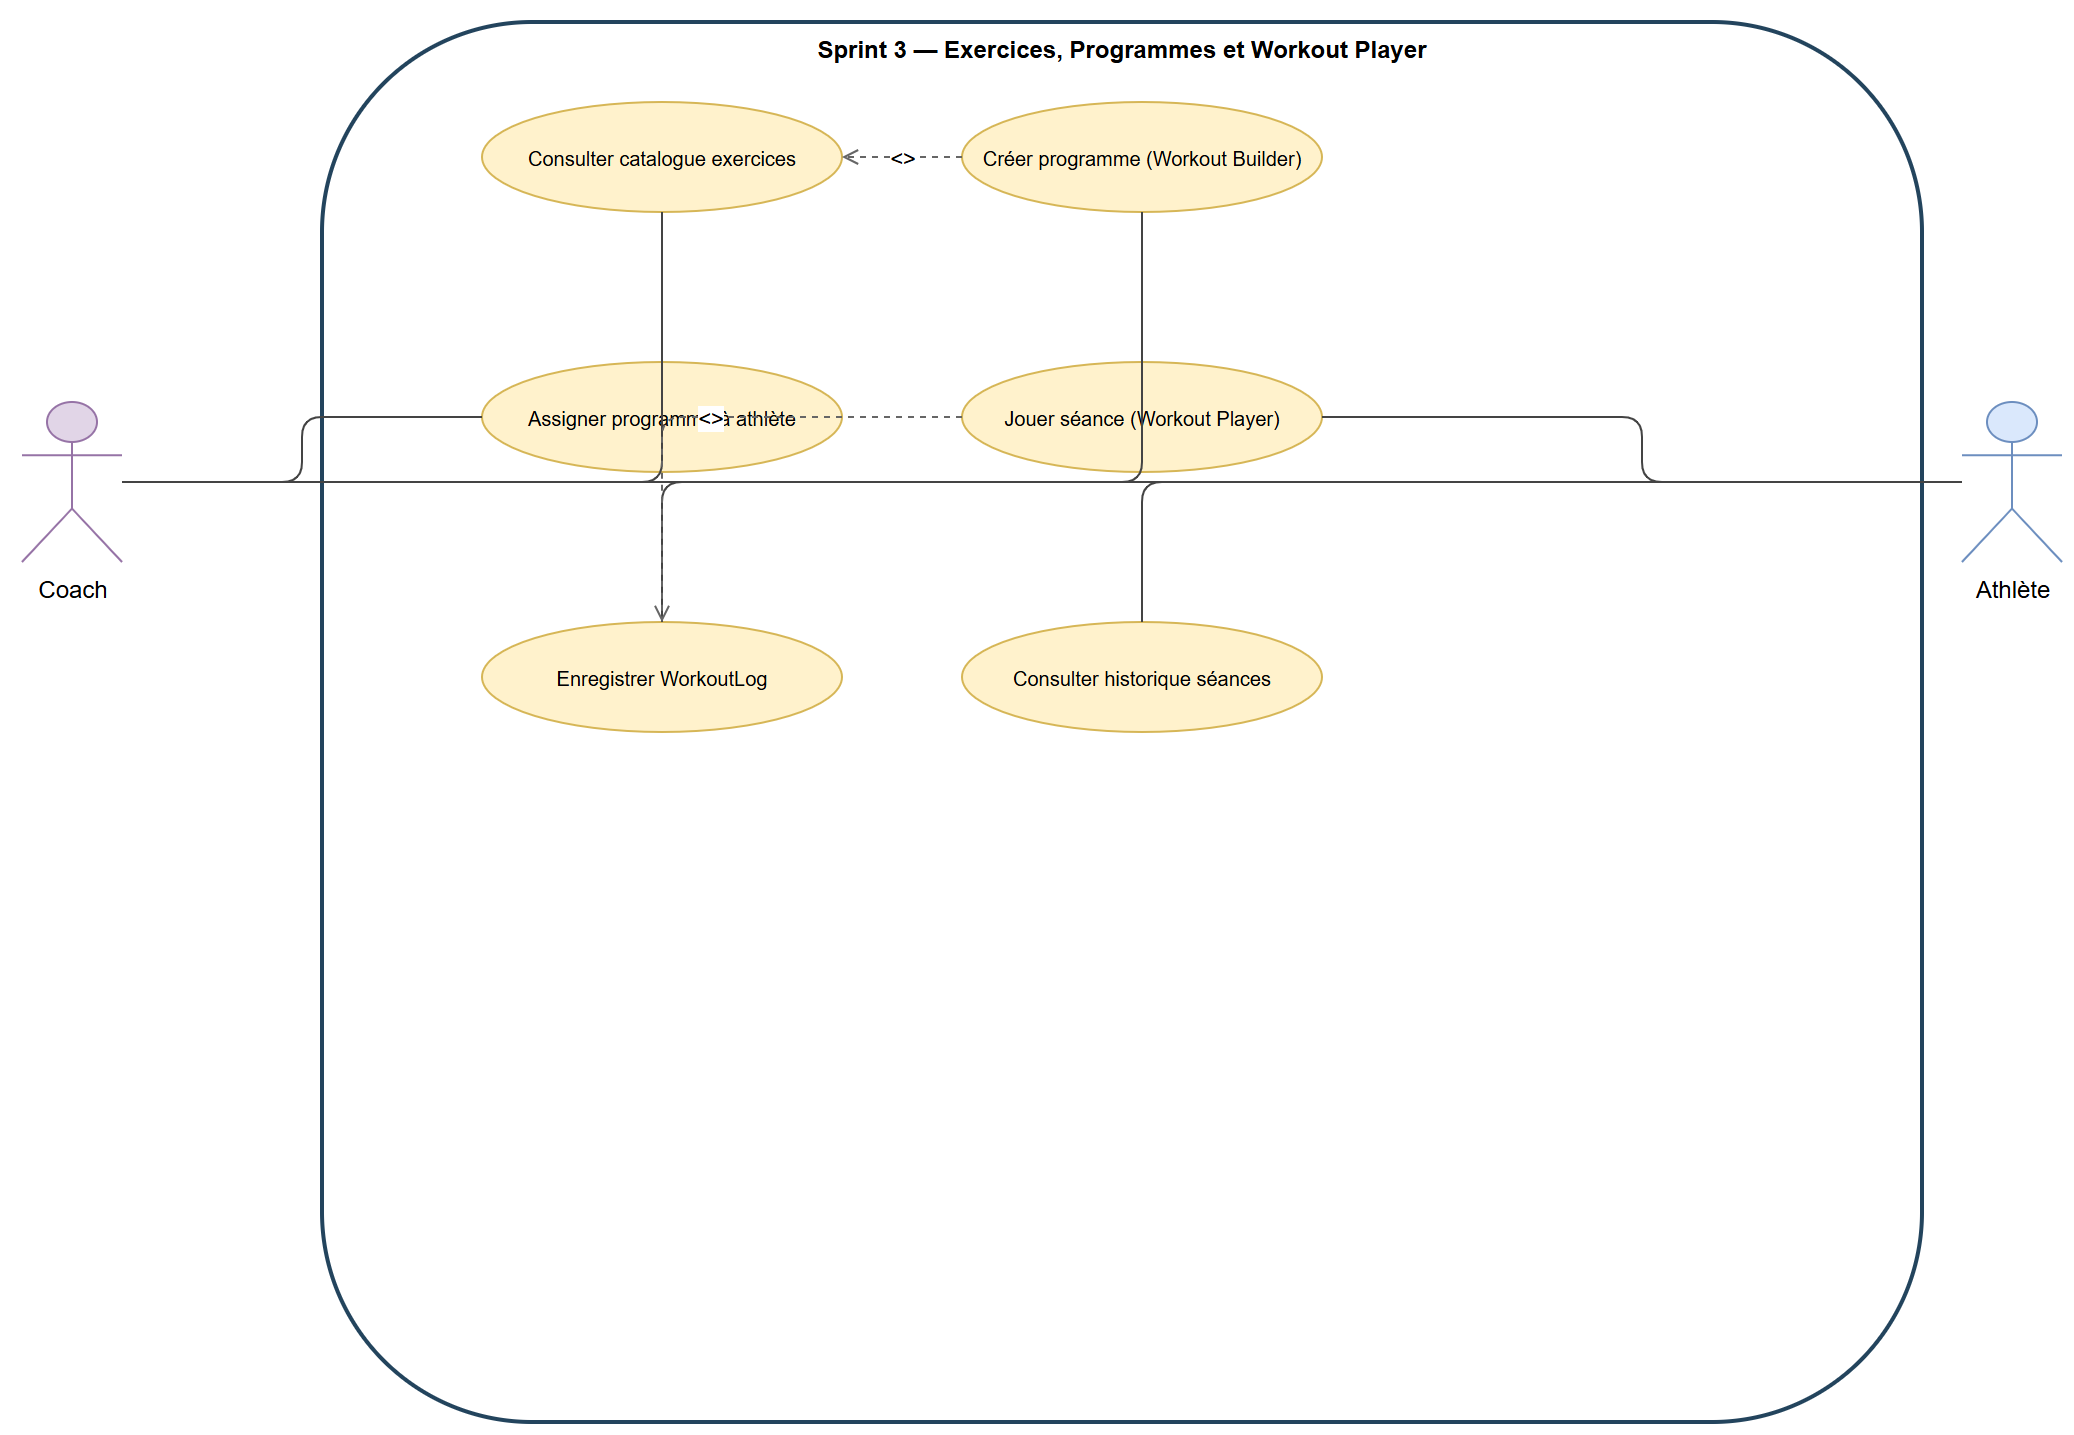
\includegraphics[width=0.85\textwidth]{diagrams/use case sprint 3.png}
\caption{Diagramme des cas d'utilisation - Sprint 3}
\end{figure}

\subsection{Diagramme de classes (Sprint 3)}
Le modèle de données s'élargit une dernière fois pour accueillir les historiques de messagerie (\texttt{Message}, \texttt{Conversation}), les entités d'administration (rôle Admin), et les tables d'audit pour stocker les requêtes formulées à l'IA (\texttt{AILog}).

%[Note : Ajoutez l'image exportée depuis Draw.io dans le dossier diagrams/ avec ce nom]
\begin{figure}[H]
\centering
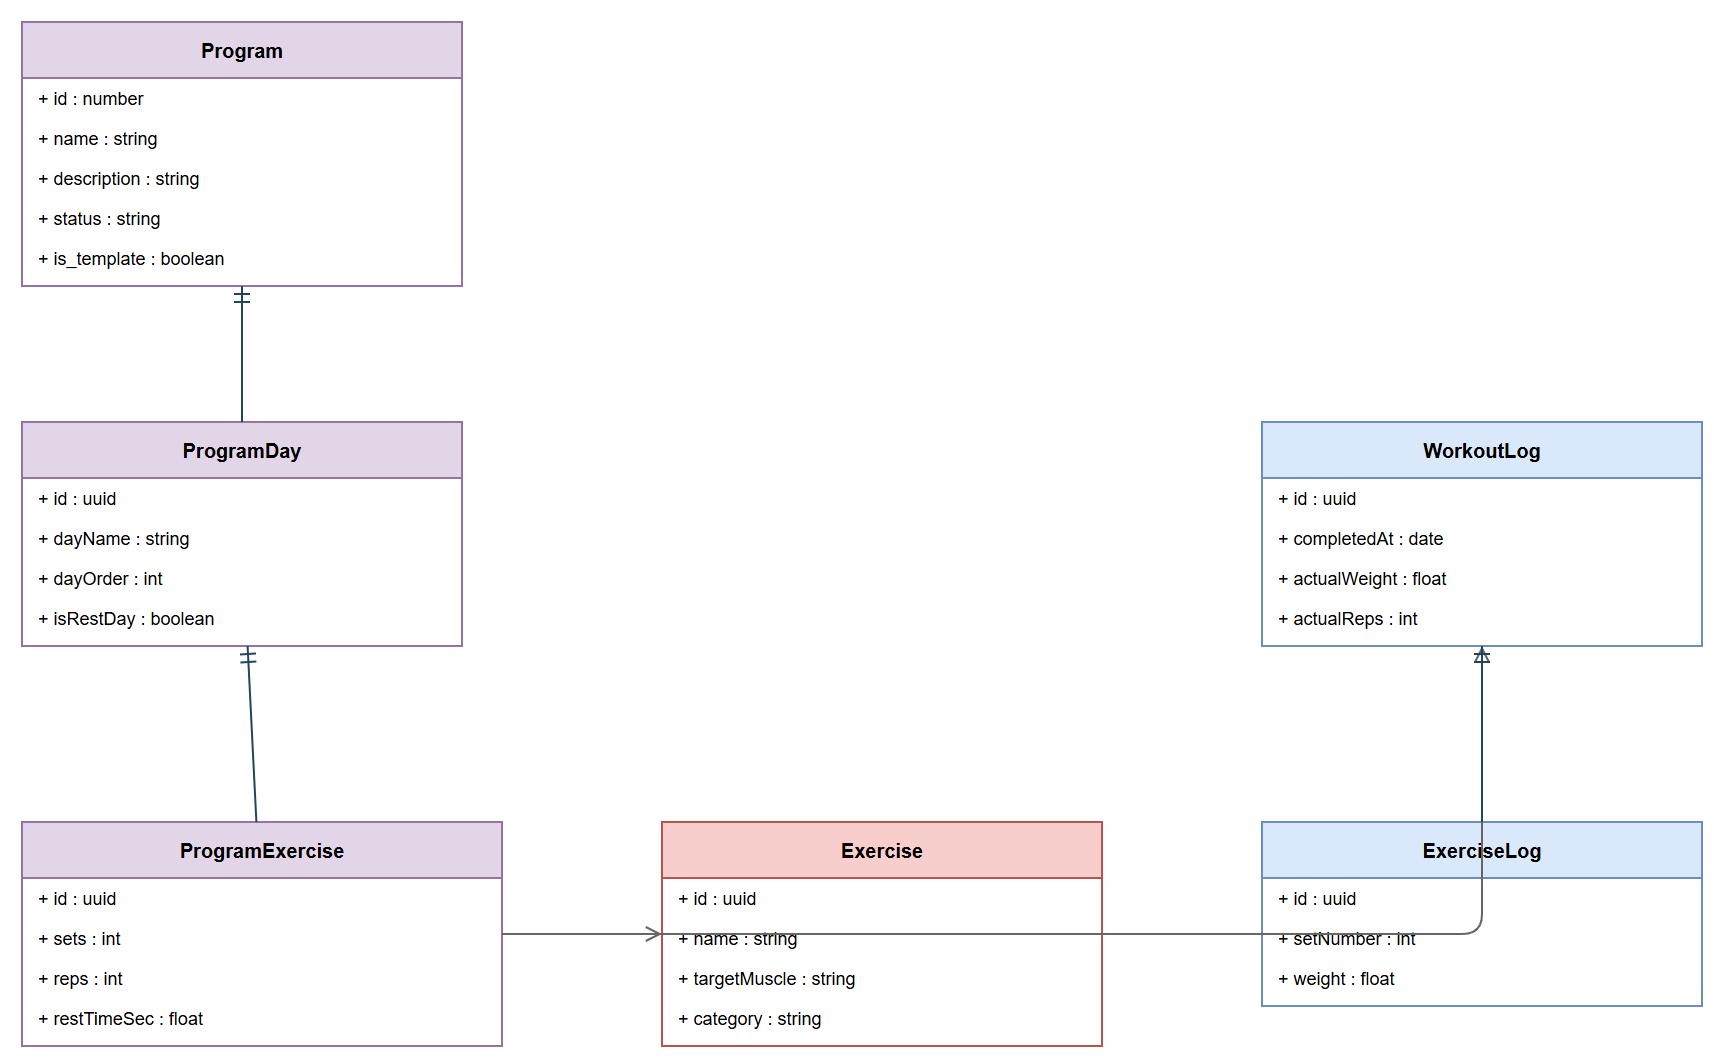
\includegraphics[width=1\textwidth]{diagrams/classe sprint 3.png}
\caption{Diagramme de classes - Sprint 3}
\end{figure}

\subsection{Diagramme de séquence : Messagerie Temps Réel}
Ce diagramme est particulièrement complexe car il illustre une double condition. Lorsqu'un message est envoyé, le serveur Node.js l'enregistre dans PostgreSQL. Ensuite, il vérifie si le destinataire est actuellement connecté au socket (en ligne). Si oui, le message est émis directement via \texttt{Socket.io}. Si non (hors ligne), le serveur déclenche l'API Firebase pour envoyer une notification push sur l'écran verrouillé du smartphone de l'athlète.

%[Note : Ajoutez l'image exportée depuis PlantUML dans le dossier diagrams/ avec ce nom]
\begin{figure}[H]
\centering
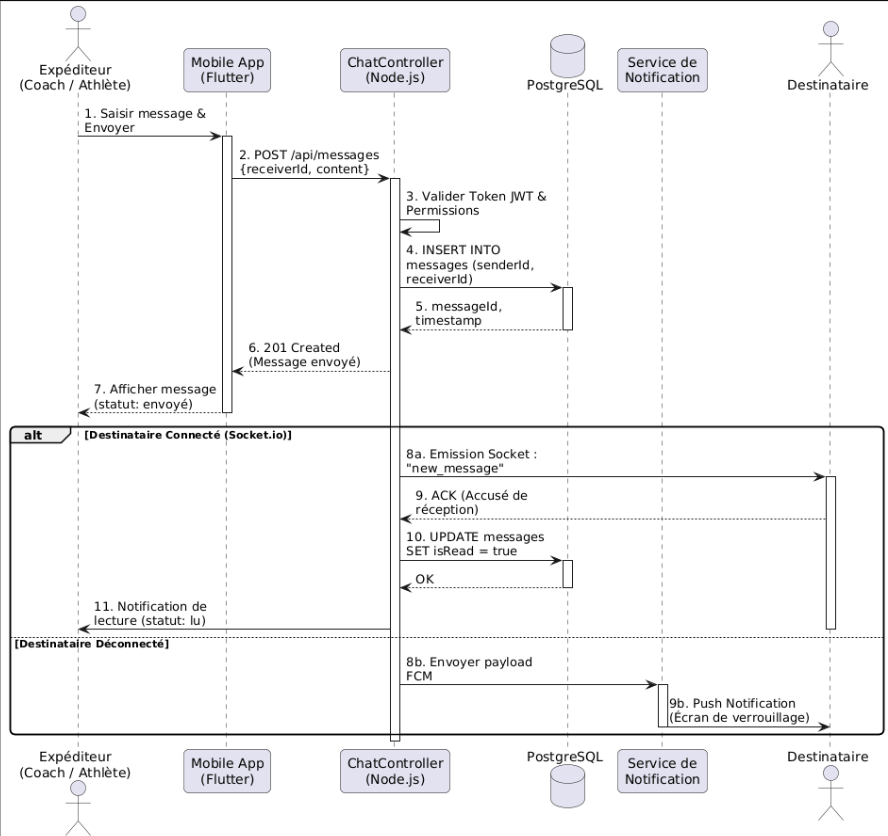
\includegraphics[width=0.9\textwidth]{diagrams/sequence sprint 3.png}
\caption{Diagramme de séquence : Messagerie en Temps Réel et Notifications}
\end{figure}

\section{Réalisation technique : La Messagerie Temps Réel}

\subsection{Le défi du Temps Réel (WebSockets vs HTTP)}
Le protocole HTTP classique, utilisé dans les sprints précédents, est unidirectionnel (le client demande, le serveur répond). Pour une messagerie, si l'on utilisait HTTP, l'application Flutter devrait demander toutes les secondes au serveur : "Y a-t-il un nouveau message ?" (technique du \textit{Long Polling}), ce qui viderait la batterie du téléphone et saturerait le serveur.

Nous avons donc implémenté le protocole \textbf{WebSocket} via la bibliothèque \texttt{Socket.io}. Une fois l'utilisateur connecté, un "tunnel" persistant est ouvert entre le smartphone et Node.js.

\subsection{Implémentation Node.js (Socket.io)}
Côté serveur, nous avons créé une passerelle (Gateway). Lorsqu'un client se connecte, nous l'ajoutons à une "Room" (chambre) correspondant à son ID. Ainsi, les messages envoyés à cette Room ne parviennent qu'à lui.

\begin{lstlisting}[language=JavaScript, caption={Passerelle WebSockets avec Node.js}, label={lst:socket_io}]
io.on('connection', (socket) => {
  console.log(`Utilisateur connecte : ${socket.id}`);
  
  // L'utilisateur rejoint sa salle privee basee sur son ID
  socket.on('join', (userId) => {
    socket.join(userId);
  });

  // Interception de l'envoi d'un message
  socket.on('sendMessage', async (data) => {
    const { senderId, receiverId, content } = data;
    
    // 1. Sauvegarde en base de donnees via TypeORM
    await chatService.saveMessage(senderId, receiverId, content);
    
    // 2. Emission en temps reel dans la salle du destinataire
    io.to(receiverId).emit('receiveMessage', {
      senderId,
      content,
      timestamp: new Date()
    });
  });
});
\end{lstlisting}

Sur l'application Flutter, la vue \textit{ChatScreen} s'abonne à l'événement `receiveMessage`. Dès réception, l'interface utilisateur appelle \texttt{setState} (ou l'équivalent BLoC) pour ajouter la nouvelle bulle de texte à l'écran instantanément, le tout avec une fluidité remarquable.

\section{Intégration du Tableau de Bord Web (Angular)}
Jusqu'à présent, toutes les interfaces étaient mobiles (Flutter). Cependant, pour gérer la plateforme globale de CoachingApp, l'administrateur a besoin d'une interface bureautique puissante. Nous avons choisi le framework Angular (v16+).

\subsection{Architecture des Composants Angular}
L'application Angular a été structurée en \textit{Modules} chargés de manière paresseuse (Lazy Loading) pour accélérer le premier rendu (First Contentful Paint).
\begin{itemize}
    \item \textbf{SidebarComponent :} Une barre latérale persistante permettant la navigation entre le Dashboard, la liste des Utilisateurs, et le Catalogue d'Exercices.
    \item \textbf{StatsComponent :} Utilisation de la librairie \texttt{Chart.js} (ou \texttt{Ng2-charts}) pour afficher des graphiques à barres sur l'évolution du nombre d'inscriptions.
    \item \textbf{ExerciseManagerComponent :} Un tableau interactif (Angular Material Data-Table) permettant à l'Admin d'ajouter (via un formulaire modal réactif) ou de supprimer des exercices du catalogue global, évitant ainsi que la base ne soit polluée par des doublons créés par les coachs.
\end{itemize}

\section{L'innovation technologique : Intelligence Artificielle}
L'un des objectifs "Could Have" de notre backlog était l'intégration de l'IA. Nous avons interfacé le serveur Node.js avec l'API \textbf{Gemini} de Google.

\subsection{Mécanique du Prompt Engineering}
L'IA ne prend pas le contrôle de l'application, elle agit comme un "Copilote" pour le coach et l'athlète.
Lorsqu'un utilisateur demande un conseil (ex: "Je me suis blessé à l'épaule, par quoi remplacer le développé couché ?"), le serveur construit un contexte masqué (Prompt Engineering) très précis avant de l'envoyer à Gemini :

\textit{"Tu es un coach sportif expert en biomécanique. L'utilisateur te pose cette question : [Question]. Réponds en maximum 3 phrases, en proposant 2 exercices de substitution sécuritaires, formatés en liste à puces."}

Le retour de Gemini est ensuite parsé par Node.js et affiché à l'utilisateur. Cette fonctionnalité réduit le temps de réponse du coach humain pour des questions génériques, et offre un service 24/7 à l'athlète.

\section{Résolution des bugs et Débogage}
Le Sprint 3, en raison de sa nature intégratrice, a été source de plusieurs défis techniques qui ont été documentés et résolus :
\begin{itemize}
    \item \textbf{Conflits de fusion Git (Merge Conflicts) :} La parallélisation du développement Flutter et Angular a généré des conflits sur le backend lors de l'ajout des routes de messagerie. Ces conflits ont été résolus de manière sécurisée en analysant l'arbre de commit.
    \item \textbf{Résolution des hôtes dynamiques (CORS \& IP) :} Lors des tests sur l'émulateur Android, l'application Flutter ne pouvait pas contacter le serveur Node.js sur \texttt{localhost}. Nous avons reconfiguré le client réseau pour pointer dynamiquement vers l'adresse IP locale de la machine hôte (\texttt{10.0.2.2} sur émulateur) et nous avons paramétré le middleware \texttt{cors()} d'Express pour autoriser les requêtes entrantes de l'application Angular.
\end{itemize}

\section{Conclusion}
Le Sprint 3 clôture la phase de développement logiciel de "CoachingApp". L'ajout des protocoles temps réel a transformé l'application statique en un écosystème vivant. L'application Angular donne tout le pouvoir nécessaire à l'administrateur, et l'intégration de l'IA (Gemini) place notre solution à la pointe de l'innovation. Dans le chapitre suivant (Chapitre 6), nous aborderons la phase de qualification de notre produit fini : les stratégies de tests logiciels, les pratiques de sécurité adoptées, et le déploiement de la solution (DevOps).
